\documentclass{article} % For LaTeX2e
\usepackage{nips13submit_e,times}
\usepackage{hyperref}
\usepackage{url}
\usepackage{graphicx}
\usepackage{adjustbox}
\usepackage{subcaption}
\graphicspath{{images/}}
%\documentstyle[nips13submit_09,times,art10]{article} % For LaTeX 2.09

\nipsfinalcopy % Uncomment for camera-ready version

\begin{document}

\title{Reddit Comment Generator}
\author{Braulio Chavez \\
  \texttt{braulioc@stanford.edu}}
\maketitle

\begin{abstract}
In this work I describe the implementation of a recurrent neural network (RNN)
to solve the problem of automatic generation of logical comments for a specific
context. The RNN makes use of LSTM cells to help keep long term data
dependencies, improving the performance of the model. For completeness I
compared the training evaluation of the LSTM cell vs the GRU cell under the
same conditions. Then I discuss the reactions that the generated comments got
from the Reddit community and how to improve the model to give it more context
and logic accuracy.
\end{abstract}

\section{Introduction}
Recurrent neural networks (RNN) have been used in a wide array of machine
learning problems. They are known to be a generative model which is a
particularly interesting property. Recently there have been various attemps to
increase the creativity of these models. These approaches are applied to
generate a varied ammount of media like images, music or poems.

In this project I make use of the generative properties of the RNN to try to
atomatize the generation of comments especific to a provided context. The
applications of this are many: FAQ answering, forum like discussion, chatbots
that help accomplish a task, gmail's autoreply feature.

The potential of this is huge, it can create be a whole new human computer
interaction paradigm on how users deal with technology. If implemented correctly
people won't even be able to discern a bot from a human on the other side of the
conversation (Turing test). This applies to any form of communication. Companies
wouldn't need to spend as many resources to generate a valuable product or
experience to their customers, think of customer service and internal processes,
even increase the usefulnes and intelligence of their current products.

The approach to solve this problem was to use already proved RNN language
models. I used the help of LSTMs to help alleviate the long term data dependecy
loss issue, this practice improved the performance of the mode. In order to have
a baseline I also experimented with a GRU which in practical terms it is a
modified LSTM with different keep and forget functions and internal mechanisms
which I'll describe later. Once these two models were trained I evaluated them
with perplexity. You can think of perplexity as a measure of how perplex or
surprised is the model of comparing the results it created with a validation
dataset.

%TODO: ADD PERPLEXITY FORMULA


\section{Background/Related Work}
RNNs, LSTMs, GRU

\section{Approach}
After some experimentation (described in the next section) with different
hyperparameter configurations, and by comparing the use of LSTM and GRU cells. I
arrived to the following language model used for comment generation. The model
is a two hidden layer RNN with LSTM cells to help with the long term data
dependency loss problem. Each hidden layer has 200 nodes. You can see a graphic
representation in figure NN.

%TODO: ADD MY MODEL'S FIGURE REPRESENTATION.

The model can be represented by the following equations:

%TODO: ADD MODELS EQUATIONS.

The evaluation of the model was with a technical metric: perplexity, and by
engagement metrics: users' replies and upvotes.

\section{Experiment}
The dataset used in the experiment was 31 GB of an entire month's of reddit
comments. It has comment's metadata such as: score, subreddit, body and author.
I sectioned it to use a single subreddit (theme/topic). I decided to use the
``funny'' subreddit, which is one of the most popular subreddits. This subset
arrived to 450 MB of comments. Then to bias the model towards better quality
comments pre-evaluated by Reddit's community with the score field, I filtered
the comments to only keep the ones with score bigger than 10 (see
figure~\ref{fig:datasetsection}).  After this sectioning the dataset used for
training was about 13\% of the comments for the ``funny'' subreddit. Then I
generated a file to contain all of the comment's body, did a further separation
to create a train, test and validation datasets with 80\%, 10\% and 10\%
original body file size correspondingly.

\begin{figure}[h]
\centering
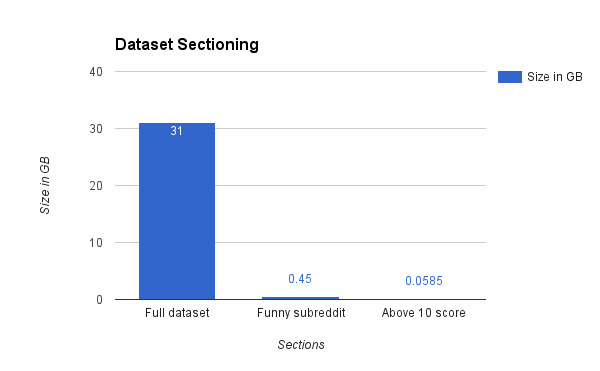
\includegraphics[scale=0.5]{dataset_sectioning}
\caption{Dataset sectioning.}
\label{fig:datasetsection}
\end{figure}
%TODO: Insert body dataset sectioninig grap for train, test and validation.

With the dataset ready I proceeded to train two models. One with LSTM and one
with GRU cells. This helped me compare the two models and choose the one that
performed the beter based solely on perplexity. I used two set of hyperparameter
configuration to train the models. You can see the hyperparameter sets used in
Table~\ref{table:hyperparameters}.

\begin{table}[h]
\caption{Used hyperparameter configurations for testing.}
\label{table:hyperparameters}
\centering
\begin{tabular}{lll}
\multicolumn{1}{c}{\bf Parameter}  &\multicolumn{1}{c}{\bf Small}
&\multicolumn{1}{c}{\bf Medium}
\\ \hline \\
batch\_size         &64         &64 \\
embed\_size         &50         &50 \\
hidden\_size        &100        &200 \\
num\_steps          &10         &20 \\
max\_epochs         &16         &26 \\
early\_stoping      &2          &2 \\
dropout             &0.5        &0.5 \\
learning\_rate      &0.001      &0.001 \\
num\_layers         &2          &2 \\
\end{tabular}
\end{table}

One of the main differences in both set of hyperparameters was the increase of
the hidden\_size parameter. By increasing it I arrived to better performance in
perplexity in both models. You can see the comparison of performance of both
models on figure~\ref{fig:perplexity}.

\begin{figure}[h]
\centering
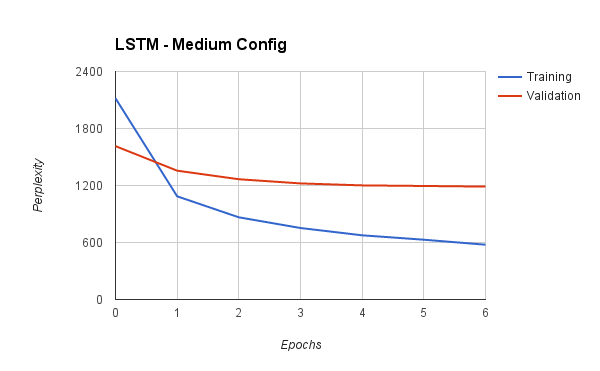
\includegraphics[scale=0.5]{lstm_medium_config}
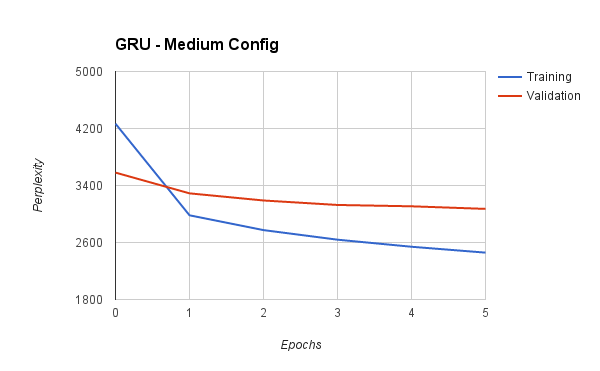
\includegraphics[scale=0.5]{gru_medium_config}
\caption{LSTM vs GRU models in training and validation perplexity.}
\label{fig:perplexity}
\end{figure}

We can clearly see that the model using LSTM cells was better than the one using
GRU cells at the given task with the same parameters. Given that conclusion I
decided to use the LSTM model's to generate test sentences. To test the quality
of the generated sentences I used a substring of the test dataset and used it as
a seed to generate a new sentence by the model. You can see the results in
figure NN.

%TODO: Insert a table with the test generated sentences compared with the test
%data.

To distribute the comments generated by my RNN I created a Reddit account called
Roy\_Nexus. I deliberatelly avoided to give any clear indication that this was
a bot, just to see people's reactions to it.

The bot worked as follows: It retrieved the top result of the feed ``rising''
under the subreddit ``funny''.  The decision to select this specific feed was
because it has posts that are not yet popular but have the potential to be at
the front page, by posting in here the bot had a chance of being relevant in the
case of selecting a future popular post. Once the bot had downloaded the
comment's information, it used the comment's title to give it as a seed of the
RNN's generative function. This way I provided some context to the RNN in hopes
of receiving back a sentence that was within the boundaries of the theme. Once
the RNN gave the output words, the bot uploaded them in a comment under the
previously selected post. Then the program slept for 15 minutes before repeating
the whole process again. The bot never commented twice on the same post.

The reaction obtained by the community was very clear: the comments generated by
the RNN were mostly non-sense or out of context. This resulted in a negative
response measured by the score the content received and by replies saying things
like ``are you having a stroke?'' or ``somebody has a case of Google translate
it seems''. You can see some screenshots of the generated comments on
figure~\ref{fig:comments}.
And you can see the some of the replies on figure~\ref{fig:replies}. Notice the
reply of the user that identified what I was doing to generate the sentences.

\begin{figure}[h]
\centering

\includegraphics[scale=0.5]{comment2}

\includegraphics[scale=0.5]{comment3}

\includegraphics[scale=0.5]{comment1}
\caption{Sample of the generated comments.}
\label{fig:comments}
\end{figure}

\begin{figure}[h]
\centering

\includegraphics[scale=0.5]{reply1}

\includegraphics[scale=0.5]{reply2}

\includegraphics[scale=0.5]{reply4}

\includegraphics[scale=0.5]{reply5}
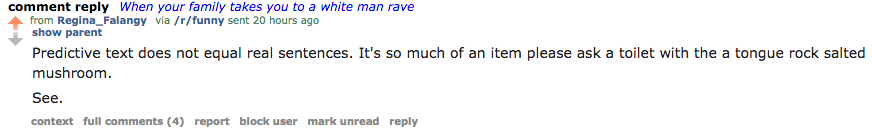
\includegraphics[scale=0.5]{reply3}
\caption{Sample of the replies by users.}
\label{fig:replies}
\end{figure}

After some days of publishing content on Reddit the the bot got tracked down and
banned from the subreddit ``funny'' by the moderators, giving end to the
experiment. On Table~\ref{table:engagement} you can see a summary of the number
of comments, replies and final comment score the bot got when finished the
experiment.

%TODO: Insert table summarizing the number of comments, replies and final
%comment score the bot obtained.
\begin{table}[t]
\caption{Engagement metrics.}
\label{table:engagement}
\begin{center}
\begin{tabular}{ll}
\multicolumn{1}{c}{\bf Concept}  &\multicolumn{1}{c}{\bf Value}
\\ \hline \\
Comments         &41 \\
Replies          &20 \\
Score            &-65 \\
\end{tabular}
\end{center}
\end{table}

\section{Conclusion}
After such a sudden forced end of my experiment. I concluded that the RNN didn't
have any sufficient consideration for the context of which it was being asked to
generate text. The title seed provided wasn't enough to guide the RNN to an
specific theme, much less to a set of themes. This task proved to be a very hard
problem.

I also think that the perplexity metric can be improved by first using more
data to train the model, second giving it more time to train and third
increasing the size of the hidden layer (as experiments concluded).

For furter extensions it would be illustrative to use a Gated Feedback RNN (GF-RNN),
this model had shown to be superior to the basic stacked RNN-LSTM, RNN-GRU
models in previous experiments and are promising. Is also interesting to mix
different models to aid in the problem of context and sentence understanding.
For example, integrating to a syntactic parser, that works by passing the input
sentences to tag each word with a part-of-speech (POS) tag that describes the
word's syntactic function, and determines the syntactic relationship between
words in the sentence, represented by a tree (see figure NN). This will help to
understand the input and output sentence of the RNN.

%TODO: insert parse tree

\section{References}

\end{document}
